
\section{Đề số 12}
\graphicspath{{./img/}}
\begin{bt} 
    \hfill
	\begin{enumerate}[a.]
		\item Tìm $x$ biết: $\quad \frac{1}{2016}: 2015 x=-\frac{1}{2015}$.
        \item Tìm các giá trị nguyên của $n$ để phân số $\mathrm{M}=\frac{3 n-1}{n-1}$ có giá trị là số nguyên.
        \item Tính giá trị của biểu thức: $N=x y^2 z^3+x^2 y^3 z^4+x^3 y^4 z^5+\ldots+x^{2014} y^{2015} z^{2016}$ tại: $\mathrm{x}=-1 ; \mathrm{y}=-1 ; \mathrm{z}=-1$
	\end{enumerate}
	\loigiai{
		\begin{enumerate}
			\item $\frac{1}{2016}: 2015 x=-\frac{1}{2015} \\
				  \frac{1}{2016.2015} x=\frac{-1}{2015} \\
				  x=\frac{-1}{2015}: \frac{1}{2016.2015}=-2016 \\
				  \text {Vậy } x=-2016$
			\item $\mathrm{M}=\frac{3 n-1}{n-1}$ có giá trị là số nguyên $\Rightarrow 3 n-1 \vdots n-1$\\
			$\Rightarrow 3(n-1)+2 \vdots n-1 \Rightarrow 2 \vdots n-1 \Rightarrow n-1 \in U^{\prime}(2)=\{-1 ; 1 ;-2 ; 2\}$\\
			Ta có bảng:\\ 
			\begin{table}[h]
				\begin{tabular}{lllll}
				\multicolumn{1}{l|}{n-1} & -1 & 1 & -2 & 2 \\ \hline
				\multicolumn{1}{l|}{n}   & 0  & 2 & -1 & 3 \\
				\end{tabular}
				\end{table}
				\\
			Thử lại ta có $n \in\{0 ; 2 ;-1 ; 3\}$ thì $\mathrm{M}$ nhận giá trị nguyên.
			\item Ta có : $\mathrm{N}=\mathrm{xyz} \cdot \mathrm{yz}^2+\mathrm{x}^2 \mathrm{y}^2 \mathrm{z}^2 \cdot \mathrm{yz}^2+\mathrm{x}^3 \mathrm{y}^3 \mathrm{z}^3 \cdot \mathrm{yz}^2+\ldots+\mathrm{x}^{2014} \mathrm{y}^{2014} \mathrm{z}^{2014} \cdot \mathrm{yz}^2$\\ Thay $\mathrm{y}=1 ; \mathrm{z}=-1$ ta được:\\
			$N =-x y z-x^2 y^2 z^2-x^3 y^3 z^3-\ldots-x^{2014} y^{2014} z^{2014} \\
	        =-(x y z)-(x y z)^2-(x y z)^3-\ldots-(x y z)^{2014} .$\\
			Thay $x y z=-1$ được:\\
			$\mathrm{N}=1-1+1-1+\ldots+1-1=0 \\
			\text {Vậy } \mathrm{N}=0 .$
		\end{enumerate}
	} 
\end{bt}

\begin{bt}
	\hfill
	\begin{enumerate}[a.]
		\item Cho dãy tỉ số bằng nhau $\frac{2 b z-3 c y}{a}=\frac{3 c x-a z}{2 b}=\frac{a y-2 b x}{3 c}$. Chứng minh: $\frac{x}{a}=\frac{y}{2 b}=\frac{z}{3 c}$
        \item Tìm tất cả các số tự nhiên $m, n$ sao cho : $2^m+2015=|n-2016|+n-2016$.
	\end{enumerate}
	\loigiai{
		\begin{enumerate}
			\item
				$\frac{2 b z-3 c y}{a}=\frac{3 c x-a z}{2 b}=\frac{a y-2 b x}{3 c} \\
				\Leftrightarrow \frac{2 a b z-3 a c y}{a^2}=\frac{6 b c x-2 a b z}{4 b^2}=\frac{3 a c y-6 b c x}{9 c^2} \\
				= \frac{2 a b z-3 a c y+6 b c x-2 a b z+3 a c y-6 b c x}{a^2+4 b^2+9 c^2}=0 \\
				\Rightarrow 2 b z-3 c y=0 \Rightarrow \frac{z}{3 c}=\frac{y}{2 b}(1) \\
				\Rightarrow 3 c x-a z=0 \Rightarrow \frac{x}{a}=\frac{z}{3 c}(2) ; \text { Từ (1) và (2) suy ra: } \frac{x}{a}=\frac{y}{2 b}=\frac{z}{3 c}$
			\item Nhận xét:\\
			$\text {-Với } x \geq 0 \text { thì }|x|+x=2 x \\
			\text {-Với } x<0 \text { thì }|x|+x=0 \text {. }$\\
			Do đó $|\mathrm{x}|+\mathrm{x}$ luôn là số chẵn với $\forall \mathrm{x} \in \mathrm{Z}$.\\
			Áp dụng nhận xét trên thì $|n-2016|+\mathrm{n}-2016$ là số chẵn với $\mathrm{n}-2016 \in \mathrm{Z}$.\\
            Suy ra $2^{\mathrm{m}}+2015$ là số chẵn $\Rightarrow 2^{\mathrm{m}}$ lẻ $\Leftrightarrow \mathrm{m}=0$.\\
            Khi đó $|\mathrm{n}-2016|+\mathrm{n}-2016=2016$\\
            + Nếu $\mathrm{n}<2016$, ta có - $(\mathrm{n}-2016)+\mathrm{n}-2016=2016 \Leftrightarrow 0=2016$ (loại)\\
            + Nếu $n \geq 2016$, ta có $2(n-2016)=2016 \Leftrightarrow n-2016=1008 \Leftrightarrow n=3024$ (thỏa mãn)\\
            Vậy $(m ; n)=(0 ; 3024)$
		\end{enumerate}
	} 
\end{bt}

\begin{bt}
	\hfill
	\begin{enumerate}[a.]
		\item Tìm giá trị nhỏ nhất của biểu thức $\mathrm{P}=|x-2015|+|x-2016|+|x-2017|$.
        \item Cho bốn số nguyên dương khác nhau thỏa mãn tổng của hai số bất kì chia hết cho 2 và tổng của ba số bất kì chia hết cho 3 . Tính giá trị nhỏ nhất của tổng bốn số này ?
	\end{enumerate}
	\loigiai{
		\begin{enumerate}
			\item $\mathrm{P}=|x-2015|+|2016-x|+|x-2017|=(|x-2015|+|2017-x|)+|x-2016|$\\
			Ta có: $|x-2015|+|2017-x| \geq|x-2015+2017-x|=2$. Dấu "=" xảy ra khi: $2015 \leq x \leq 2017$ (1)\\
			Lai có: $|x-2016| \geq 0$.\\ 
			Dấu "=" xảy ra khi $\mathrm{x}=2016$ (2).\\
			Từ (1) và (2) ta có $\mathrm{minP}=2$. Dấu " $=$ " xảy ra khi $x=2016$
			\item Nhận xét : Bốn số phải có cùng số dư khi chia cho 2 và 3 . Để có tổng nhỏ nhất, mỗi trong hai số dư này là 1 .\\
			Từ đó ta có các số $1,7,13$ và 19 . Tổng của chúng là : $1+7+13+19=40$.
		\end{enumerate}
	}
\end{bt}

\begin{bt}
    Cho tam giác $\mathrm{ABC}$ cân tại $\mathrm{A}, \mathrm{BH}$ vuông góc $\mathrm{AC}$ tại $\mathrm{H}$. Trên cạnh $\mathrm{BC}$ lấy điểm $M$ bất kì ( khác $B$ và $C$ ). Gọi $D, E, F$ là chân đường vuông góc hạ từ $M$ đến $A B, A C$, $\mathrm{BH}$.
    \begin{enumerate}
        \item Chứng $\operatorname{minh} \triangle \mathrm{DBM}=\triangle \mathrm{FMB}$.
        \item Chứng minh khi $\mathrm{M}$ chạy trên cạnh $\mathrm{BC}$ thì tổng $\mathrm{MD}+\mathrm{ME}$ có giá trị không đổi.
        \item Trên tia đối của tia $C A$ lấy điểm $\mathrm{K}$ sao cho $\mathrm{CK}=\mathrm{EH}$. Chứng minh $\mathrm{BC}$ đi qua trung điểm của DK.
    \end{enumerate}
\loigiai{
	$$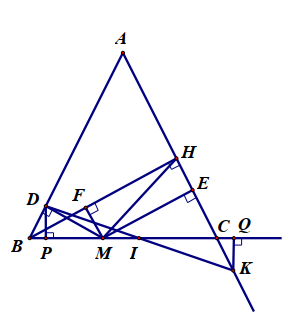
\includegraphics[width=0.4\textwidth]{12-4-lg.png}$$
	\begin{enumerate}
		\item $\text {Chứng minh được } \Delta \mathrm{DBM}=\Delta \mathrm{FMB} \text { (ch-gn) }$
		\item Theo câu a ta có: $\Delta \mathrm{DBM}=\Delta \mathrm{FMB}($ ch-gn $) \Rightarrow \mathrm{MD}=\mathrm{BF}$ (2 cạnh tương ứng)\\
		+) Chứng minh: $\Delta \mathrm{MFH}=\Delta \mathrm{HEM} \Rightarrow \mathrm{ME}=\mathrm{FH}$ (2 cạnh tương ứng)
		$(2)$\\
		Từ (1) và (2) suy ra: $\mathrm{MD}+\mathrm{ME}=\mathrm{BF}+\mathrm{FH}=\mathrm{BH}$\\
		BH không đổi $\Rightarrow \mathrm{MD}+\mathrm{ME}$ không đổi (đpcm)
		\item Vẽ $D P \perp B C$ tại $P, K Q \perp B C$ tại $Q$, gọi I là giao điểm của $D K$ và $B C$\\
		+) Chứng minh : $\mathrm{BD}=\mathrm{FM}=\mathrm{EH}=\mathrm{CK}$\\
		+) Chứng minh : $\triangle \mathrm{BDP}=\triangle \mathrm{CKQ}$ (ch-gn) $\Rightarrow \mathrm{DP}=\mathrm{KQ}$ (cạnh tương ứng)\\
		$+)$ Chứng minh: $\mathrm{IDP}=\mathrm{IKQ} \Rightarrow \Delta \mathrm{DPI}=\Delta \mathrm{KQI}(\mathrm{g}-\mathrm{c}-\mathrm{g}) \Rightarrow \mathrm{ID}=\mathrm{IK}$(đpcm)\\
	\end{enumerate}
}
\end{bt}

\begin{bt}
   Có sáu túi lân lượt chứa $18,19,21,23,25$ và $34$ bóng. Một túi chỉ chứa bóng đỏ trong khi năm túi kia chỉ chứa bóng xanh. Bạn Toán lấy ba túi, bạn Học lấy hai túi. Túi còn lại chứa bóng đỏ. Biết lúc này bạn Toán có số bóng xanh gấp đôi số bóng xanh của bạn Học. Tìm số bóng đỏ trong túi còn lại.
\loigiai{
	Tông số bóng trong 6 túi là : $18+19+21+23+25+34=140$
    Vì số bóng của Toán gấp hai lần số bóng của học nên tổng số bóng của hai bạn là bội của 3 . Ta có : 140 chia 3 bằng 46 dư 2. Do đó số bóng đỏ cũng là số chia 3 dư 2 .\\
    Trong sáu số đã cho chỉ có 23 chia 3 dư 2, đó chính là số bóng đỏ trong túi còn lại. Từ đó ta tìm được số bóng của Toán là : $18+21=39$. Số bóng của học là : $19+25+34=78$.
}
\end{bt}